
\chapter{Methods}
\label{Chapter3}

\section{Context}

To cope with the complexity of metagenomes, the size of the reference databases and the resulting uncertainty in read assignments, early abundance estimation tools like Bracken \cite{lu_bracken:_2017} and MEGAN \cite{huson_megan_2007} did not provide the abundances for each reference genome, but only for taxonomic clusters like species, genus or phylum.

This approach introduces a bias due to the structure of the phylogenetic or taxonomic tree, in which some species may be over-represented, others are still subject to adjustments, and in certain cases the definition is not coherent: in the Mycobacterium genus, for instance, Mycobacterium Bovis and Mycobacterium Tuberculosis are classified as two different species even though their genomes are characterized by 99.5\% similarity, while the threshold used for species separation is normally way lower \cite{garnier_complete_2003}.

Furthermore, the technological improvements in read sequencing provide increased resolution for the metagenomic samples, by generating either short high quality reads with error rate <1\% as with Illumina and Sanger machines, or long reads with higher error rates as with ONT and PacBio. The detail of the information in these sequences allow, with sufficiently high coverage, to map at least some of the reads in the metagenome to the exact reference genome they are likely to come from, when they are present in the database.

Nevertheless, due to the high similarity among the reference genomes of the same species, most reads, especially those associated to the core genome, will still map to multiple references equally well. Therefore reads assigned to subsets of the reference database need to be probabilistically redistributed to each genome.

Several tools including Bracken and GASiC build their model for read redistribution on top of the estimated similarity of the reference genomes. In Bracken, every $k$-mer of each reference is mapped to the index using the Kraken algorithm, and the frequency with which $k$-mers are assigned to internal nodes of the taxonomic tree are used to estimate the probability that a read of the metagenome assigned to such internal nodes originates from each reference in its subtree using Bayes' theorem. In this model, the $k$-mer length $k$ should match the length of the reads in the sample, but the technology used to sequence the metagenome is not taken into account, reducing the robustness of the method. By fixing $k$, it also makes it unfit for machines producing reads of variable length like ONT. Furthermore, by assigning every $k$-mer of the database it increases the computational burden and the risk of overfitting.

Gasic \cite{lindner_metagenomic_2013} introduced a new approach based on read simulation. Read simulators provide realistic sequences by using probabilistic models built from the results of different sequencing technology. This allows the abundance estimation to be independent from the sequencing technology, which evolves at a fast pace. Reads are simulated from each reference genome with a low coverage and with parameters resembling those of the metagenomic sample, then aligned to the references using a fast aligner like BWA \cite{li_aligning_2013} or Bowtie \cite{langmead_fast_2012}. Reads mapped to multiple reference genomes are used to build a similarity matrix which is specific to the sequencing technology and the aligner used in the real experiment, and a LASSO linear model is built on top of it.

Inspired by these two methods, we developed an abundance estimator for alignment-free tools, which has been integrated in the program ProPhyle. Exploiting ProPhyle's lossless $k$-mer index, producing assignments which are more accurate than Kraken's (see figure \ref{fig:mult_ass}), we decided to focus on the genome level and to make use of the model introduced by Gasic for alignment tools.

\subsection{Desired Properties}

A major problem with Bracken and other abundance estimators is the amount of false positives in their output. Indeed, due to the size of modern metagenomic read sets, which may contain up to billions of sequences, it happens frequently that reference genomes which are known not to be present in the sample still have non-zero assignment counts. This happens either because those genomes are highly similar to other references which indeed are present in the sample, or because those reads are generated from a novel strain which is not included in the database and has no better representative, in which case the assignment will probably have a low score.

While dealing with the second issue requires a preprocessing step to filter out poor quality assignments, the first one can be solved by defining thresholds for the number (or percentage) of specific assignments that a given genome needs to get to be considered as present, where specific means that no other reference genome is matched equally well, as it is done in Bracken. Nevertheless, this solution is once again affected by the uneven representation of species in the database, where well-studied species like human pathogens include hundreds or thousands of representative genomes while others only have few representatives. In the first case, the probability that a read matches an exact genome instead of an entire cluster decreases considerably, since most $k$-mers are shared by the whole cluster.

The solution adopted in Gasic, using LASSO \cite{tibshirani_regression_1996} to regularize the linear redistribution model and filter out false positives, also has some drawbacks. The major issue appears in the presence of highly similar clusters in the reference database: if the genomes in the cluster all have a comparable amount of assignment, the $L_1$ regularization penalty will be likely to select one of them at random and filter out the others.

To address the issue of Gasic, we used the Elastic Net regressor. Elastic Net combines the $L_1$ regularization used in LASSO and the $L_2$ regularization (also called Tikhonov or Ridge regularization). The Elastic Net can be seen as a generalization of LASSO, and it introduces a so-called ``grouping effect'', avoiding the random selection of highly correlated genomes as it happens with LASSO. Furthermore, the path with which predictors are set to 0 by its variable selection property is more stable than LASSO's when regularization parameters change (figure \ref{fig:enet_vs_lasso}). This feature guarantees consistent results when using different parameters to fit metagenomes of different complexity.

\subsection{Linear Regression}

Linear regression is a linear approach to modelling the relationship between a scalar response (or dependent variable) and one or more explanatory variables (or independent variables) \cite{noauthor_linear_2018}. The relationship between these two sets of variables is modeled with linear functions of the kind:
\begin{equation*}
    y_i = \beta_0 + \beta_1 x_{i1} + \dots + \beta_p x_{ip} + \varepsilon_i ~,~~ i = 1, \dots , n
\end{equation*}
where $y_i$ is the response variable, the vector $\vec{x_i} = \{x_{i1}, \dots, x_{ip} \}$ contains the $p$ explanatory variables for $y_i$, the vector $\boldsymbol{\beta} = \{\beta_0, \dots, \beta_p \}$ is the vector of regression coefficients including the intercept term $\beta_0$, and $\varepsilon_i$ is an error term which accounts for noise in the data. In matrix notation, the model can be expressed as:
\begin{equation*}
    \vec{y} = \boldsymbol{X}\boldsymbol{\beta} + \boldsymbol{\varepsilon}
\end{equation*}

The standard method for estimating the regression coefficients is Ordinary Least Squares (OLS). This method consists in minimizing the sum of the squares of the differences between the observed dependent variable and those predicted by the linear function \cite{noauthor_linear_2018}. This is equivalent to the optimization of the following function:
\begin{equation*}
    \boldsymbol{\hat{\beta}} = \argmin_{\beta}{\norm{\vec{y} - \boldsymbol{X}\boldsymbol{\beta}}_2^2}
\end{equation*}
Under the assumption that the error vector $\boldsymbol{\varepsilon}$ is normally distributed, OLS is therefore equivalent to the Maximum Likelihood (ML) estimator \cite{noauthor_linear_2018}.

In the context of metagenomic abundances, the observed assignment counts can be modelled as the dependent variables of a linear model, while the regression coefficient could represent the unknown abundances of the reference genomes in the sample, to be estimated using some explanatory matrix. In our case, the explanatory variables will be measures of similarity of the reference genomes. Due to the similarities between genomes of the same species being very high, and to the increasing number of genomes used as references in metagenomic experiments, it is unrealistic to expect this model to fit the data by simply using OLS. In fact, in this case most of the genomes will be considered as present by the model, since the reads in the sample will be mapped to several references, but only few of them will actually be present. To address this issue, we use a model which performs both regularization and variable selection: the Elastic Net.

\subsection{The Elastic Net}

To avoid overfitting a linear model, or to improve its performance when the problem is ill-posed, the technique of regularization is often used. In a regularized model, a regularization term is included in the minimization we have already seen for OLS:
\begin{equation*}
    \boldsymbol{\hat{\beta}} = \argmin_{\beta}{\norm{\vec{y} - \boldsymbol{X}\boldsymbol{\beta}}_2^2} + \norm{\boldsymbol{\Gamma}\boldsymbol{\beta}}_2^2
\end{equation*}
where $\boldsymbol{\Gamma}$, called Tikhonov matrix, is usually chosen as a multiple of the identity matrix. Although introducing this $L_2$ regularization penalty, so called because it uses the $l^2$ norm or Euclidean distance, has a beneficial effect on overfitting issues by shrinking large regression coefficients, an $L_1$ regularization penalty can be used in order to enforce their sparsity, thus performing variable selection. This technique, known as LASSO \cite{tibshirani_regression_1996}, has been already proved to be an effective solution for metagenomics in \cite{lindner_metagenomic_2013}.

While the most intuitive way to enforce sparsity is by using the $l^0$ norm, i.e. the number of non-zero coefficients, this would break the convexity of the objective function to optimize, making it an NP-hard problem \cite{donoho_compressed_2006}. Nevertheless, the $l^1$ norm has been shown to approximate $l^0$, therefore providing similar performance without loosing the convexity property.
On the other hand, the $l^2$ norm does not provide the same effect: the intuition of the reason in 2D is in the figure \ref{fig:reg_norms}. Let us consider the problem as a constrained optimization problem:
\begin{equation*}
    \boldsymbol{\hat{\beta}} = \argmin_{\beta}{\norm{\vec{y} - \boldsymbol{X}\boldsymbol{\beta}}_2^2}~~\text{s.t.}~~f(\beta) \leq t
\end{equation*}
for $f=\norm{\cdot}_1$ and $f=\norm{\cdot}_2^2$. In the first case, the likelihood of a convex object which lies tangent to the boundary to encounter a ``corner'' is higher than in the second case, where the rotational invariance of the ($n$-)sphere contrasts this property.

\begin{figure}
  \caption{Optimization space for the $L_1$, $L_2$ and Elastic Net regularizations in 2D. Adapted from \cite{noauthor_lasso_nodate}}
  \centering
    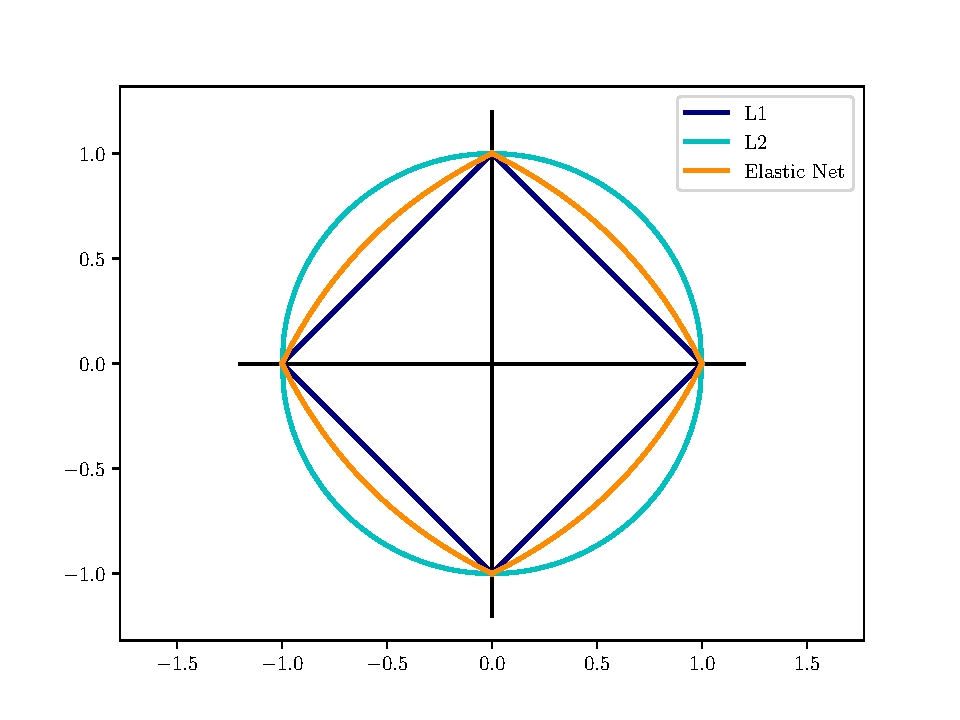
\includegraphics[width=1\textwidth]{Figures/reg_norms.pdf}
  \label{fig:reg_norms}
\end{figure}

\begin{figure}
  \caption{Example of regularization path for the coefficients of the LASSO and Elastic Net methods on the same instance. Varying the regularization weight $\alpha$ results in smoother transitions for the Elastic Net. Adapted from \cite{noauthor_lasso_nodate}}
  \centering
    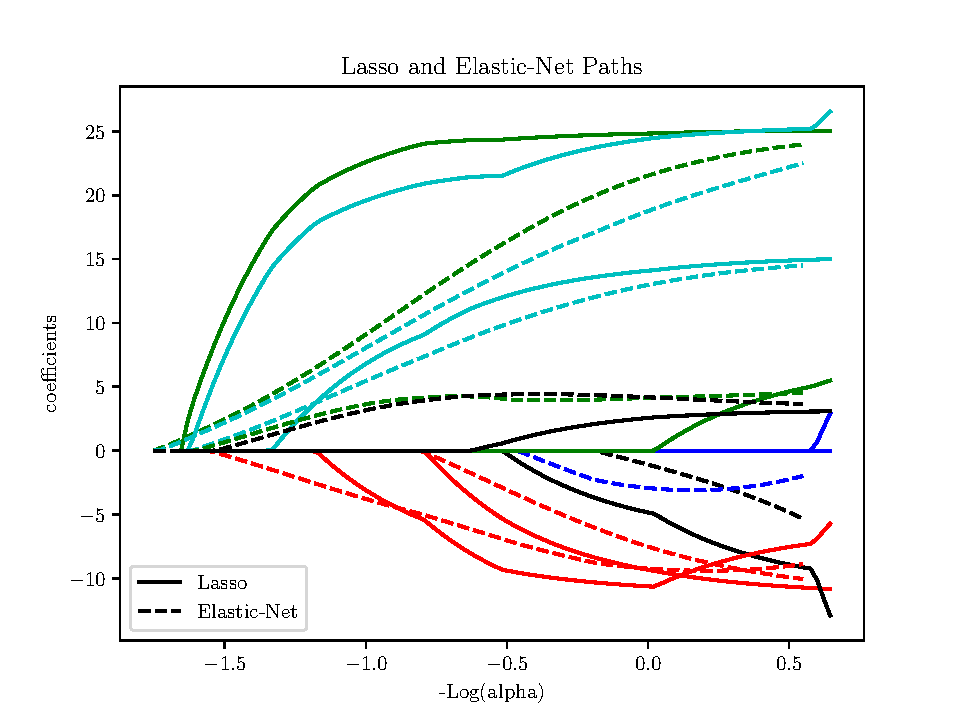
\includegraphics[width=1\textwidth]{Figures/enet_vs_lasso.pdf}
  \label{fig:enet_vs_lasso}
\end{figure}

While both $L_1$ and $L_2$ regularization penalties have desirable properties for our application, respectively the sparsity and the shrinking of the regression coefficients, they both come with some drawbacks. The LASSO has proven to be extremely variable because of its inherent discreteness, as shown in \cite{breiman_heuristics_1996}. On the other hand, the Tikhonov regression does not provide the desired variable selection property, since using the $l^2$ norm it keeps all the predictors in the model. It has also been observed that in a variety of applications, each technique may perform better than the other.

The Elastic Net addresses the issues above by linearly combining the $L_1$ and $L_2$ regularization penalties. The resulting objective function to optimize is:
\begin{equation*}
    \boldsymbol{\hat{\beta}} = \argmin_{\beta}{\norm{\vec{y} - \boldsymbol{X}\boldsymbol{\beta}}_2^2} + \lambda_1 \norm{\boldsymbol{\beta}}_1 + \lambda_2\norm{\boldsymbol{\beta}}_2^2
\end{equation*}

The greatest advantage provided by this method is its grouping effect. As shown in Theorem 1 of \cite{zou_regularization_2005}, this property tends to give similar regression coefficients to highly correlated variables. This is particularly important when fitting metagenomic data of high complexity, where several strains of the same species may be present in the sample. In such situation, LASSO would be likely to only select one such variable at random \cite{zou_regularization_2005}.

% \subsection{Solving Linear Models}
% \begin{itemize}
%     \item coordinate descent
%     \item SVM reduction
% \end{itemize}
% A technique frequently used for solving linear models, including the sklearn python library implementation we use for the benchmarks of this model, is coordinate descent. Coordinate descent algorithms fix the majority of components in the regression coefficients vector at their value from the current iteration, and approximately minimize the objective function for the non-fixed coordinates. The subproblems are of lower dimension, thus easier to solve than the original problem \textbf{[ref cd]}. These algorithms are especially fit for computational statistics and machine learning applications, where the cost of computing one component of the gradient is low and there is no need for extreme accuracy.

% \begin{itemize}
%     \item algo for regularization term
%     \item cyclic vs random
% \end{itemize}

\section{Model}

Inspired by the LASSO linear model defined in \cite{lindner_metagenomic_2013} and the improvements in its successor \cite{fischer_abundance_2017}, we have designed a model to estimate metagenomic abundances from read assignments, focusing especially on the properties of the assignments of the metagenomic classifier ProPhyle.

Thanks to the lossless property of ProPhyle's index, its read assignments have a higher resolution than other alignment-free methods (cf. \ref{Chapter2}). Even though metagenomic reads can still be assigned to internal nodes of the taxonomic tree, this has a different meaning with respect to the assignments of e.g. Kraken: for ProPhyle, a read is assigned to an internal node if and only if every genome in its subtree has the same assignment score (i.e. shares the same number of $k$-mers with the read); for Kraken, this may happen if two or more, possibly distant genomes have the same score, in which case the tie would be solved by assigning the read to their lowest common ancestor (LCA) instead of providing their list, or if they share every $k$-mer in the read, in which case the $k$-mers themselves would be associated to their LCA in the database, making a precise assignment impossible in the first place.

Therefore we designed a model which focuses on the genome level, and which does not take into account the structure of the taxonomic tree but only the actual similarity of the reference genomes, as it is ``perceived'' through ProPhyle's index and assignment algorithm. As introduced in \cite{lindner_metagenomic_2013}, a first simulation step is performed in order to estimate such similarities, then read assignments are optimized using an Elastic Net-based linear model.

\subsection{Model Definition}

\subsubsection{Similarity matrix estimation}
In order to estimate the similarity between each couple of reference genomes, reads are simulated from each of them and assigned to the full reference set. The similarity matrix, whose columns encode the distribution of the assignments, is built as follows:
\newpage
\begin{algorithmic}
\State $\mathbf{S} \gets \mathbb{M}_{n\times n}$
\For {ref. genome $i \in D$}
\State $s_{*i} \gets \mathbf{0}^n$
\State simulate read set $R_i$ from genome $i$
\For {read $\in R_i$}
\State $I \gets$ assign(read)~~~[$I \subseteq D_n$]
\For {$j \in I$}
\State $s_{ji}~~{+=}~~1$
\EndFor
\EndFor
$s_{*i}~~{/=}~~s_{ii}$
\EndFor
\end{algorithmic}
where $D_n$ is the reference database containing the $n$ reference genomes.

The value of $s_{ij}$ encodes the number of reads simulated from reference $j$ which map to reference $i$, divided by the number of reads which map back to a subset containing reference $j$. This represents an estimate for the similarity of genomes $(i,j)$, according to their $k$-mer composition encoded in the ProPhyle index used for the assignment.

\subsubsection{Optimization}
Let $\vec{m} = [m_1, \dots, m_n]^T$ be the vector of mappings of a sample, calculated in the very same way as a column of $\boldsymbol{S}$ (its sum will exceed the total number of reads in the sample, since a multiple assignment to subset $I$ will increment by 1 the entry of each reference genome $g_j \in I$). In order to recover the vector of true abundances $\mathbf{r} = [r_1, \dots, r_n]^T$, we need to solve the following system of linear equations:
\begin{equation*}
  \vec{m} = \boldsymbol{S} \cdot \vec{r}
\end{equation*}
with non-negativity constraints $r_i \geq 0~\forall i$. The equation corresponding to genome $i$ is:
\begin{equation*}
  m_i = r_i + \sum_{i \neq j}^n s_{ij} \cdot r_j
\end{equation*}

To estimate the solution to this system, we solve it using $\vec{r}$ as the regression coefficient vector of the Elastic Net.

\subsection{Implementation}

Simulating reads which reflect the properties of the metagenomic sample to be classified is a crucial step of the optimization pipeline: parameters like read length and error profile of the technology used to sequence the real sample may highly affect the performance of the method. For this reason, we have used the simulation framework RNFsim \cite{brinda_rnf_2016} in the implementation of this step. RNFsim includes some of the most efficient and accurate read simulators and enables reproducible and fully-parametrizable read simulation; it can also easily be extended to match the characteristics of evolving sequencing technologies. In order to obtain accurate results, the simulated reads should match the characteristics of the real data as closely as possible.

For the optimization step, we relied on the implementation of the coordinate descent algorithm for Elastic Net provided by the scikit-learn Python framework. The code\footnote{\url{https://github.com/scikit-learn/scikit-learn/blob/master/sklearn/linear_model/cd_fast.pyx}} which performs the optimization is implemented in C as a Cython extension, and provides fast and stable convergence.

At the time of writing, all the programs and scripts are publicly available in ProPhyle's Github repository\footnote{\url{https://github.com/prophyle/prophyle}} in the branch \texttt{enet\_abundances}. Every step in the pipeline described above will be integrated in the next main release of ProPhyle.

\subsection{Error estimations}

To benchmark the method we used the two following error measures, where $e_i$ and $t_i$ are respectively the estimated and true abundances of genome (or species, genus, etc.) $i$:
\begin{itemize}
  \item MAE (Mean Absolute Error):
  \begin{equation*}
    \frac{\sum_{i=1}^n |e_i - t_i|}{n}
  \end{equation*}
  \item RSS (Residual Sum of Squares):
  \begin{equation*}
    \sum_{i=1}^n (e_i - t_i)^2
  \end{equation*}
\end{itemize}

In addition to these measures of the distance between the true and estimated abundances, we focused on the false positive and false negative rates, which are arguably the most important measures in many metagenomic experiments: while slight changes in the relative abundances may be interesting for some particular applications, having a reliable list of what the sample is composed of is always a valuable information. Furthermore, we provide two measures for those rates: first, the number of FP (resp. FN), i.e. the amount of genomes which are present in the output of the programs but not in the sample (resp. present in the sample and not in the output), and secondly their relative abundance. We will show that our method achieves superior genome selection performances with respect to the other tools analyzed, while improving the error calculated with the measures above.
